\documentclass{beamer}


% Beamer settings
\usecolortheme{rose}
\beamertemplatenavigationsymbolsempty
\setbeamertemplate{footline}[frame number]

% Packages
\usepackage{amsmath}

\usepackage{pgfplots}
\usepgfplotslibrary{fillbetween}

\usepackage{minted}
\usepackage[T1]{fontenc} % Required by minted to ensure dollar signs are produced instead of pound (sterling) signs

\usepackage{multicol}

\usepackage{booktabs}


\title{OpenMP for Computational Scientists}
\subtitle{5: Programming your GPU with OpenMP}

\begin{document}

\frame{\titlepage}

%-------------------------------------------------------------------------------
\begin{frame}
\frametitle{Outline}
\begin{itemize}
  \item GPU introduction
  \item The OpenMP \mintinline{fortran}|target| directive
  \item Memory movement
\end{itemize}
\end{frame}

%-------------------------------------------------------------------------------
\begin{frame}
\frametitle{GPU performance}

\begin{columns}
\begin{column}{0.5\textwidth}
\begin{adjustbox}{max width={\textwidth}}
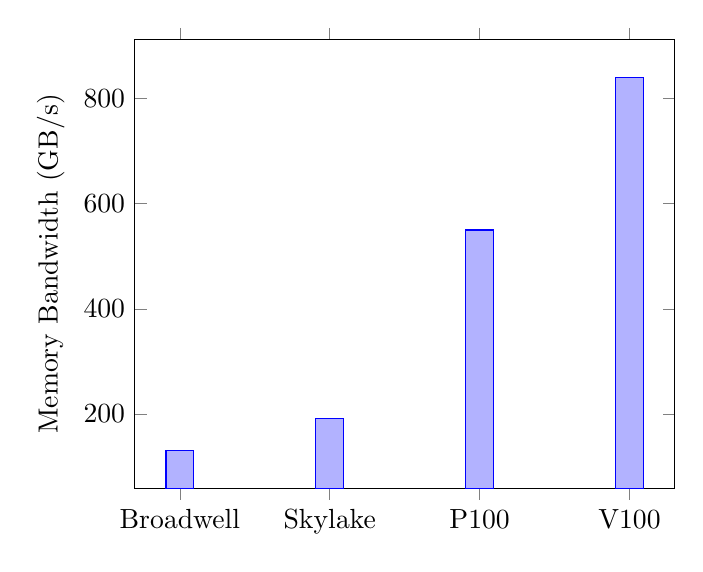
\begin{tikzpicture}
  \begin{axis}[ybar,
               symbolic x coords={Broadwell, Skylake, P100, V100},
               xtick=data,
               ylabel={Memory Bandwidth (GB/s)}]
    \addplot coordinates {(Broadwell,130) (Skylake,191) (P100,550) (V100,841)};
  \end{axis}
\end{tikzpicture}
\end{adjustbox}
\end{column}

\begin{column}{0.5\textwidth}
\begin{adjustbox}{max width={\textwidth}}
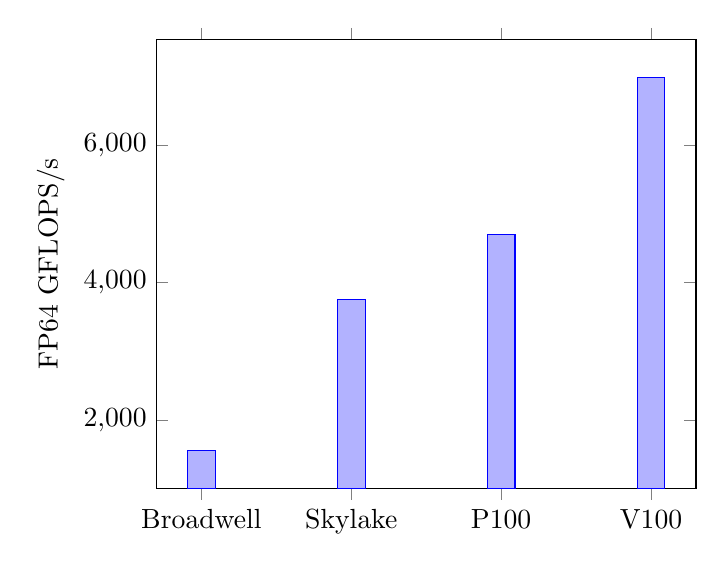
\begin{tikzpicture}
  \begin{axis}[ybar,
               symbolic x coords={Broadwell, Skylake, P100, V100},
               xtick=data,
               ylabel={FP64 GFLOPS/s}]
    \addplot coordinates {(Broadwell,1550) (Skylake,3760) (P100,4700) (V100,7000)};

  \end{axis}
\end{tikzpicture}
\end{adjustbox}
\end{column}
\end{columns}

\begin{itemize}
  \item Volta GPUs offer 4.4X memory bandwidth and 1.9X the FLOPS/s of dual-socket Skylake.
\end{itemize}

\end{frame}

%-------------------------------------------------------------------------------
\begin{frame}
\frametitle{Unlocking this potential}
\begin{itemize}
  \item GPUs made of many cores (SMs):
    \begin{itemize}
      \item V100 has 80 SMs.
      \item P100 has 56 SMs.
    \end{itemize}
  \item Each SM consists of 64 FP32 CUDA cores.
  \item CUDA cores are really organised as 2 vector units 32 wide (called warps).
\end{itemize}

\begin{block}{Take away}
GPUs are really vector-architectures made up of smaller blocks which execute together.
\end{block}
\end{frame}

%-------------------------------------------------------------------------------
\begin{frame}
\frametitle{GPUs need lots of parallelism}
\begin{itemize}
  \item GPUs are \emph{throughput optimised}, whereas CPUs are \emph{latency optimised}.
  \item Throughput optimised also called \emph{latency tolerant}.
  \item GPUs achieve this by running many operations at once, and overlapping these with each other.
  \item Hence need many (many) operations\dots
  \item A V100 has 5,120 processing elements, each needing multiple units of work to overlap.
\end{itemize}
\begin{block}{Take away}
Massive amounts of parallelism to exploit.
\end{block}
\end{frame}

%-------------------------------------------------------------------------------
\begin{frame}[fragile]
\frametitle{Device model}
\begin{itemize}
  \item OpenMP has a host/device model.
  \item Execution begins on the host CPU, with zero or more devices connected to the host.
  \item Memory spaces \emph{not} shared!
  \item Some data copied automatically, plus explicit copying.
  \item Directives are used to transfer execution to the device.
  \begin{minted}{fortran}
  !$omp target [clause [clause] ...]
  !$omp end target
  \end{minted}
  \item Host executiuon idels until target region completes (exact semantics based on tasks).
\end{itemize}

\vfill

\begin{center}
\begin{tikzpicture}
  \draw (-1,0) node {Host};
  \draw (-1,-1) node {Device};
  \draw (0,0) -- (2,0);
  \draw[dashed] (2,0) -- (3,-1);

  % GPU
  \draw (3,-1) -- (5,-1);
  \draw (3,-1.2) -- (5,-1.2);
  \draw (3,-1.4) -- (5,-1.4);
  \draw (3,-1.6) -- (5,-1.6);
  \draw (3,-0.8) -- (5,-0.8);
  \draw (3,-0.6) -- (5,-0.6);
  \draw (3,-0.4) -- (5,-0.4);

  \draw[dashed] (5,-1) -- (6,0);
  \draw[->] (6,0) -- (8,0);
\end{tikzpicture}
\end{center}
\end{frame}

%-------------------------------------------------------------------------------
\begin{frame}[fragile]
\frametitle{The target directive}
\begin{minted}{fortran}
!$omp target [clause [clause]...]
!$omp end target 
\end{minted}
\begin{itemize}
  \item Starts executing \emph{in serial} on the target device.
  \item Need other directives to expand parallelism.
  \item \mintinline{fortran}|nowait| clause:
    \begin{itemize}
      \item Allows host thread to continue working. Must synchronise later using tasks.
    \end{itemize}
  \item Other clauses mainly about memory movement, which we'll come to later.
  \item In general, you'll run loops on the device using:
  \begin{minted}[frame=single]{fortran}
  !$omp target teams distribute parallel do
  do i = 1, N
    ... ! Loop body
  end do
  !$omp end target teams distribute parallel do
  \end{minted}
\end{itemize}
\end{frame}

%-------------------------------------------------------------------------------
\begin{frame}[fragile]
\frametitle{Execution model: teams}
\begin{itemize}
  \item OpenMP \emph{threads} on a device are grouped into a \emph{team}.
  \item Can synchronise threads \emph{within} a team. \emph{Cannot} synchronise between teams.
  \item Groups of teams are called a \emph{league}.
  \item \mintinline{fortran}|target| directive offloads (serial) execution to device.
  \item \mintinline{fortran}|teams| directive creates a league of times.
  \item Master thread in each team (redundantly) executes the code.
\end{itemize}

\begin{minted}[frame=single]{fortran}
!$omp target teams 
... ! Code
!$omp end target teams
\end{minted}
\end{frame}

%-------------------------------------------------------------------------------
\begin{frame}[fragile]
\frametitle{Execution model: distribute}
\begin{itemize}
  \item Share iterations of a loop between teams.
  \item Each team gets part of the iteration space.
  \item Change default assignment with \mintinline{fortran}|dist_schedule(static)| clause. Optionally include chunk size.
  \item Still only the master thread in the team executes them.
\end{itemize}

\begin{minted}[frame=single]{fortran}
!$omp target teams distribute
do i = 1, N
... ! Code
end do
!$omp end target teams distribute
\end{minted}
\end{frame}

%-------------------------------------------------------------------------------
\begin{frame}[fragile]
\frametitle{Execution model: parallel do}
\begin{itemize}
  \item Same semantics as on the CPU!
  \item Launches threads within the team and shares iterations between threads.
  \item Note, iterations that were assigned to the team by \mintinline{fortran}|distribute| directive are shared between threads in the team.
  \item Can use the \mintinline{fortran}|schedule| clause too.
  \item Remember, can synchronise between threads in the team.
\end{itemize}

\begin{minted}[frame=single]{fortran}
!$omp target teams distribute parallel do
do i = 1, N
... ! Code
end do
!$omp end target teams distribute parallel do
\end{minted}
\end{frame}

%-------------------------------------------------------------------------------
\begin{frame}[fragile]
\frametitle{Execution example}
\begin{minted}[frame=single]{fortran}
!$omp target teams distribute parallel do
do i = 1, N
  c(i) = a(i) + b(i)
end do
!$omp end target teams distribute parallel do
\end{minted}
\end{frame}

%-------------------------------------------------------------------------------
\begin{frame}
\frametitle{NVPROF}
\end{frame}

%-------------------------------------------------------------------------------
\end{document}

